%%%%%%%%%%%%%%%%%%%%%%%%%%%%%%%%%%%%%%%%%%%%%%%%%%%%%%%%%%%%%%%%%%%%%%%%%%%%%%
%%% Sample file for MTech Project Papers for Evaluation by Supervisor and Reader
%%Skeleton LaTeX file: double column format.
%%%%%%%%%%%%%%%%%%%%%%%%%%%%%%%%%%%%%%%%%%%%%%%%%%%%%%%%%%%%
%%REMEMBER  THE PAGE SIZE RESTRICTIONS
%%Mid-term :   8 Pages
%%Final        : 16 Pages
%%%%%%%%%%%%%%%%%%%%%%%%%%%%%%%%%%%%%%%%%%%%%%%%%%%%%%%%%%%%


\documentclass{article}
\usepackage{hyperref}
\usepackage[numbers]{natbib}
\usepackage{mathtools}
\DeclarePairedDelimiter\floor{\lfloor}{\rfloor}
\usepackage{multicol}
\usepackage{graphicx,changepage}
\usepackage{amsmath}
\usepackage{caption}
\graphicspath{ {images/} }
\pagestyle{empty}
\setlength{\topmargin}{ 0.25in}
\setlength{\columnsep}{2.0pc}
\setlength{\headheight}{0.0in}
\setlength{\headsep}{0.0in}
\setlength{\oddsidemargin}{-.19in}
\setlength{\parindent}{1pc}
\textheight 8.75in
\textwidth 6.8in
\newcommand{\quotes}[1]{``#1''}
\title{\large \bf Moving beyond RNNs: Attention Networks }
\author{Sachin Mittal}

\date{}

\begin{document}

	\maketitle
    \begin{center}
        Mid-term MTech Project Report
    \end{center}
        \vskip 12pt
	\thispagestyle{empty}
	\bibliographystyle{unsrt}
	
		\begin{abstract}
		RNNs are very commomn in any sequence to sequence task and have an inherently serial structure that prevents them from being run in parallel. In RNNs are NOT invariant to distance between token, i.e. as the distance grows between input token, it becomes harder to capture dependencies between them. In this report, We study a new simple network architecture, the Transformer, based solely on attention mechanisms, and entirely  dispensing with recurrence and convolutions. Transformer \cite{DBLP:journals/corr/VaswaniSPUJGKP17} was released one year back (2017) by Google team and has shown state of the art result of that time on two machine translation tasks. Despite achieveing state of art result, it fail to generalize in many tasks (e.g. copying strings or even simple logical inference when the string or formula lengths exceed those observed at training time), however those tasks can be handeled by RNNs with ease. 
		 In later section we have described a recently proposed architecture by Google team, Universal Transformer\cite{dehghani2018universal}. Experiments in original paper shows that  Universal Transformer is able to genralise on various algorithmic tasks and language understanding tasks. UT outperforms both Transformer and LSTM in machine translation, and also achieves a new state of the art on the bAbI linguistic reasoning task\cite{weston2015aicomplete}.
	\end{abstract}	
	
	\hfill \\
	
	\begin{multicols}{2}
	\section{INTRODUCTION}
Sequence to sequence learning has been successful in many tasks such as machine translation, speech recognition and text summarization amongst others. A typical Encoder-Decoder model encodes the input sequence with a series of bi-directional recurrent neural networks (RNN) and generates a variable length output with another set of decoder RNNs, both of which interface via a soft-attention mechanism.
Traditionally, both the encoder and the decoder were composed of recurrent neural networks (RNNs). RNNs sequentially process the input tokens $(x_1, x_2, ... , x_n)$  into hidden encodings $(z_1, z_2, ... , z_n)$ , then sequentially generate the output tokens $(y_1, y_2, ... , y_m)$. There are two main problems with this approach.

One is the sequential nature of RNNs. $z_i$  depends on $z_{i-1}$ , meaning it is impossible to compute $z_i$  and $z_{i-1}$  in parallel. The ability to process inputs in parallel is very important in deep learning since we normally use GPUs which work far better for parallel inputs. The other is the difficulty of learning long-range dependencies in the network. 
\\ In this report we mainly present three architectures- the Transformer, Universal Transformer and Semi-Autoregressive transformer those relying entirely on an attention mechanism to draw global dependencies between input and output and  allows significantly more parallelization. The later 2 architectures have Transformer as base model and modified it, so we have presented Transformer in detalied.
		
	\section{Transformer}
The Transformer $-$ a model that completely rely on attention to increase the training speed of model. To Illustrate details about Transformer we have used machine translation as example.


\begin{center}
\captionsetup{type=figure}
        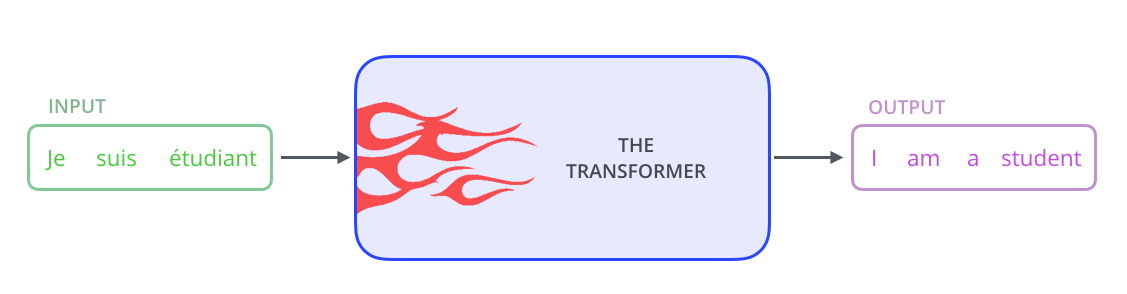
\includegraphics[width=.47\textwidth]{the_transformer_blackbox.png}
        \captionof{figure}{Transformer as black box for machine translation }
\end{center}

Transformer is encoder decoder architecture but unlike traditional encoder-decoders It attends all of the input in parallel.

\begin{center}
        \captionsetup{type=figure}
        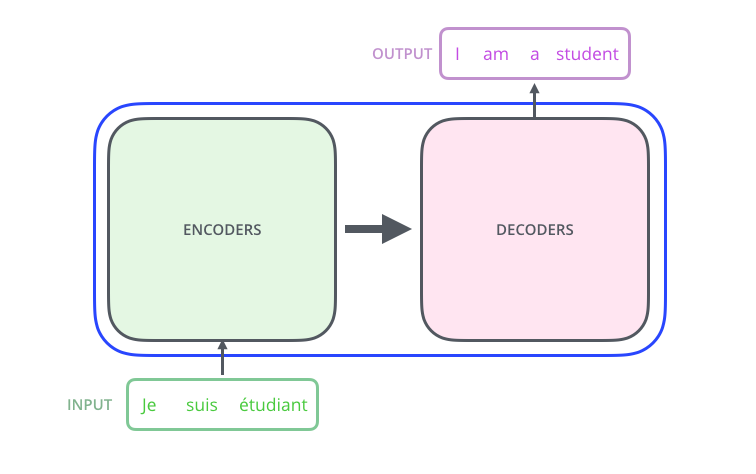
\includegraphics[width=.40\textwidth]{2.png}
        \captionof{figure}{Transformer: Encoder-Decoder }
\end{center}

Both Components (encoding and decoding) are stack of $N$ on top of each other. Each encoder consists of 2 sublayers namely, self attention and feed forward. Each of this sublayer has  layer-normalization step and residual connections before passing it to subsequent layer.

Below figure shows one encoder out of $N$ stacked encoders and zooming out sublayers of individual encoder.

\begin{center}
        \captionsetup{type=figure}
        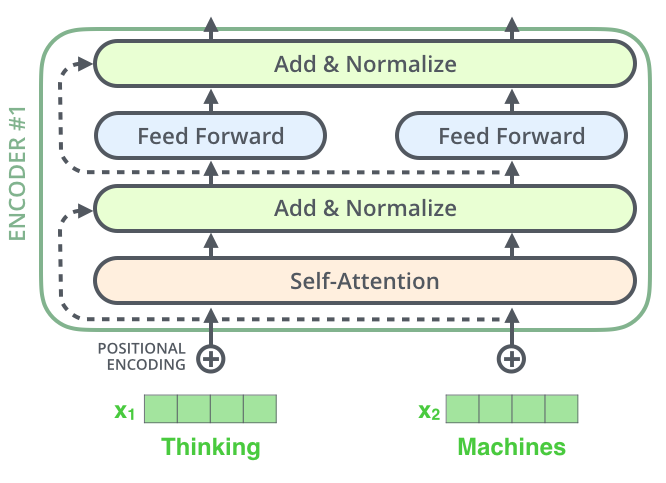
\includegraphics[width=.40\textwidth]{EncoderSublayer.png}
        \captionof{figure}{Encoder Sublayers and their interaction}
\end{center}


Now lets see both sub layers at high level.
 \subsection{Self Attention}
 The first step in calculating self attention is to create three vectors using input of encoder. Very first encoder has embedding of words as input and later encoders (in stacked encoders) has output of previous encoder as input to themselves. To genrate three vectors - query, key and value, We have three (trainable) matrices $W^Q$, $W^K$ and  $W^V$.
 Multiplying $x1$ by the $W^Q$ weight matrix produces $q1$, the "query" vector associated with that word. We end up creating a "query", a "key", and a "value" projection of each word in the input sentence.

\begin{center}
       $q_i = x_iW^Q$ \\
        $k_i = x_iW^K$\\
         $v_i = x_iW^V$
       
\end{center}
Once we have these vectors, now we calculate self-attention scores. The score determines how much focus to place on other parts of the input sentence as we encode a word at a certain position. Reason why it is called self attention is because we compare each word with its own too.

\noindent To calculate scores for $i^{th}$ word, we need to compare it against every word in sequence. We take query vector of $i^{th}$ word and key vectors of every other word and perform dot product. These dot products are supplied to softmax and later gets multiplied with value vectors.
\begin{center}
        \captionsetup{type=figure}
        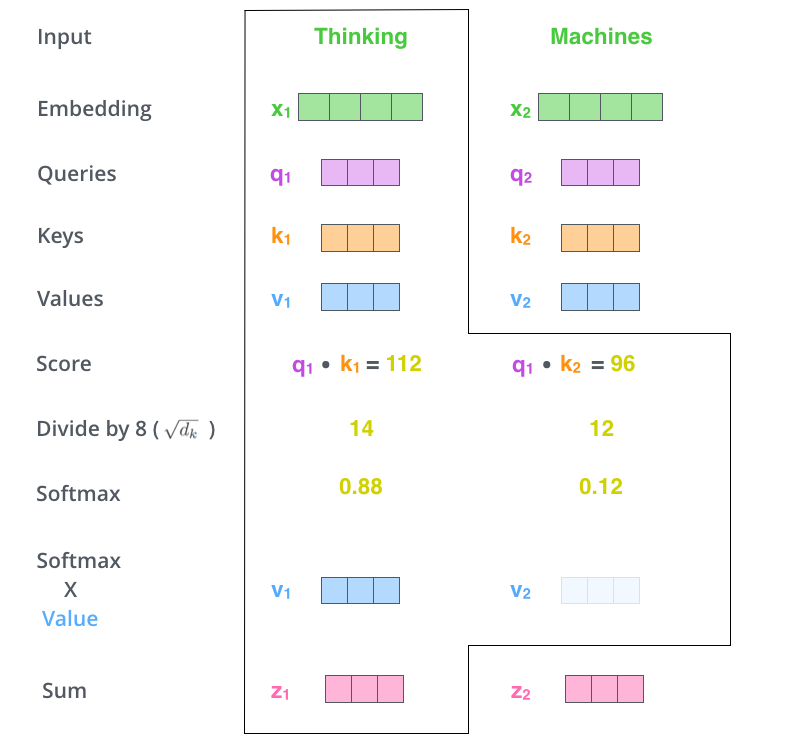
\includegraphics[width=.40\textwidth]{ZvectorSoftmax.png}
        \captionof{figure}{Attention calculation (here $z_1 =  (0.88 \times v_1) + (0.12 \times v_2)$) }
\end{center}


\noindent Since we can deal with matrices, so we can condense all calculations of $z$ vectors into matrix form- 
\begin{center}
$Z = \text{softmax}\Big( \frac{Q\times K^T}{\sqrt{d_k}} \Big)V$\\
\end{center}
where $d_k$ is the dimension of the key. The authors scale the dot product by $1/\sqrt{d_k}$ to avoid the
inputs to softmax function growing too large in magnitude.
\subsection{The core component: Multi-Head Attention}

If we only computed a single attention weighted sum of the values, it would be difficult to capture various different aspects of the input. To improve the expressive ability of the model, the Transformer uses the Multi-Head Attention block. Instead of computing a single attention pass over the values, the Multi-Head Attention computes multiple attention weighted sums – hence the name “Multi-Head” Attention.

Multi-Head Attention applies different linear transformations to the values, keys, and queries for each “head” of attention. This is illustrated in the following figure:
\begin{center}
        \captionsetup{type=figure}
        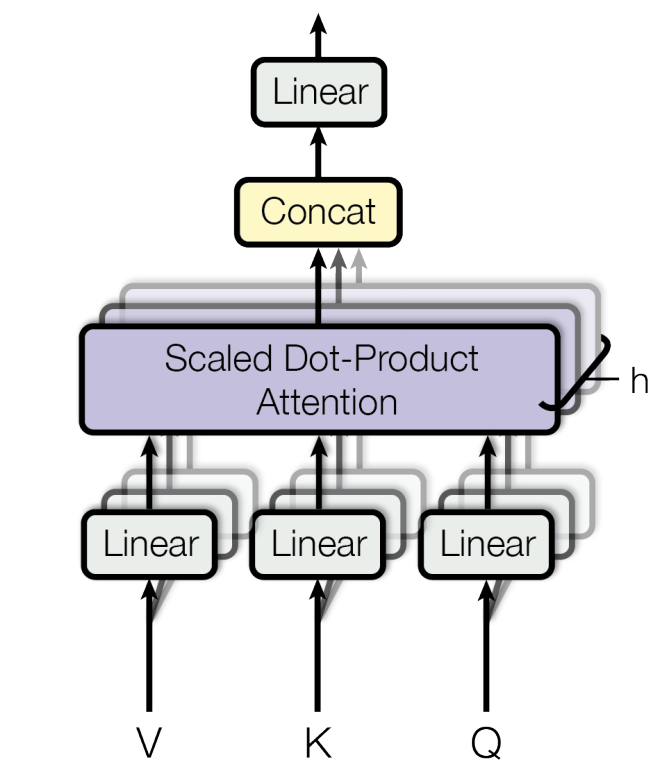
\includegraphics[width=.40\textwidth]{MultiHead.png}
        \captionof{figure}{MultiHead Attention }
\end{center}

Multihead Attention results in multiple $Z$ matrices but sublayer2 (feedforward layer) in encoder is expecting only one $Z$ matrix. We concatenate them and again perform linear projection. Following equation descibe this operation -
\begin{center}
$\text{MultiHead}(Q, K, V ) = \text{Concat} (Z_1, Z_2 \dots Z_h)W^O$
where $Z_i = \text{Attention} (XW^Q_i,XW^K_i, XW^V_i)$
\end{center}
(where $X$ is input to encoder.)

\subsection{Preserving The Order of The Sequence Using Positional Encoding}
Since we are dealing with sequential data, we need to take care of sequence in which the words are. For this purpose, Transformer uses Positional Encoding. Positional encodings explicitly encode the relative/absolute positions of the inputs as vectors and are then added to the input embeddings.
Following equation are used to compute the positional encodings:
\begin{center}
$\text{PE(pos,2i) = sin(pos/10000}^{2i/d_{model}})$\\
$\text{PE(pos,2i+1) = cos(pos/10000}^{2i/d_{model}})$
\end{center}
\noindent The idea here is that adding these values to the embeddings provides meaningful distances between the embedding vectors once they’re projected into Q/K/V vectors and during dot-product attention.
Positional embedding are only added to first encoder, later encoders has previous encoder outputs as input.

\subsection{Feed-Forward layer (Sublayer2)}
Output of attention sublayer is feeded to feedforward layer. Remember that for every input word we have output $z$ from attention sublayer. Feed-Forward layer operation can be seen as follows:- 

\begin{center}
$FFN(z) = max(0, zW_1 + b_1)W_2 + b_2$
\end{center}

\noindent Now, notice that $W_1, b_1,W_2 \text{ and } b_2$  are shared among all words in sequence. This operation can be viewed as 1D convolution operation on sequence.

\noindent We apply fully connected layer to each position each position separately and identically. This consists of two linear transformations with a ReLU activation in between.

\subsection{Decoder}

\begin{center}
        \captionsetup{type=figure}
        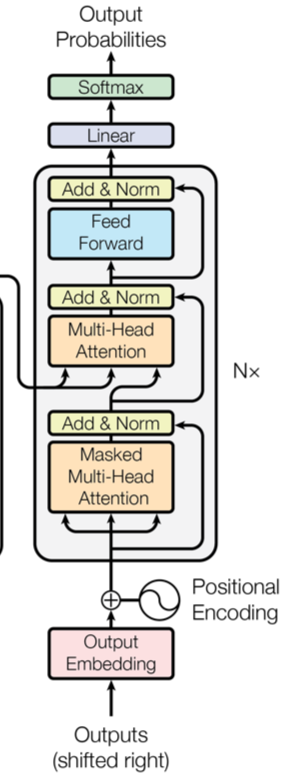
\includegraphics[height=.65\textwidth , width=.40\textwidth]{decoder.png}
        \captionof{figure}{Decoder }
        \label{decoder}
\end{center}
The decoder is very similar to the encoder but has one additional sub-layer, which is a modification of the Multi-Head Attention network, called the “masked multi-head attention” network (Figure~\ref{decoder}).
The output of the top encoder is transformed into a set of attention vectors K and V. These are to be used by each decoder in its attention sublayer which helps the decoder focus on appropriate places in the input sequence:
%%%%%%%%%%%%%  This can be followed by several other sections
    \section{Universal Transformer}
     Universal Transformers, an extension to standard Transformer which is computationally universal using a novel and efficient flavor of parallel-in-time recurrence. The Universal Transformer is built to yield stronger results across a wider range of tasks.
     
     In each step, the Universal Transformer iteratively refines its representations for all positions in the
sequence in parallel with a self-attention mechanism. The crucial change is that, It has replaced the Transformer’s fixed stack of different transformation functions with several applications of a single, parallel-in-time recurrent transformation function.


\begin{center}
$\text{MultiHeadSelfAtttention}(H) = \text{Concat} (\text{head}_1, \text{head}_2 \dots \text{head}_k)W^O$
where $\text{head}_i = \text{Attention} (HW^Q_i,HW^K_i, HW^V_i)$
\end{center}

At step t, the Universal Transformer computes revised representations $H^t \in  R^{m\times d}$ for all $m$ input positions as follows

\begin{center}
$H^t  = \text{LayerNorm}(A^{t-1})+\text{Transition}(A^t)$
\end{center}
\begin{center}
 \noindent $ A^t  = \text{LayerNorm}(H^{t-1})+\text{MultiHeadSelfAttention}(H^{t-1}+P^t)$
\end{center}

\noindent Depending on the task, Transition function is either feed forward network (similar to Transformer) or a separable
convolution. \\
$P^t$ above are two-dimensional (position, time) coordinate embeddings,

\begin{center}
$P^t_{\text{pos},2j} = sin(pos/10000^{2i/d})\bigoplus sin(t/10000^{2i/d})$
$P^t_{\text{pos},2j+1} = cos(pos/10000^{2i/d})\bigoplus cos(t/10000^{2i/d})$
\end{center}

After T steps, the final output of the Universal Transformer encoder is a matrix of d-dimensional vector representations $H^t \in  R^{m\times d}$ for the m symbols of the input sequence.


\begin{center}
        \captionsetup{type=figure}
        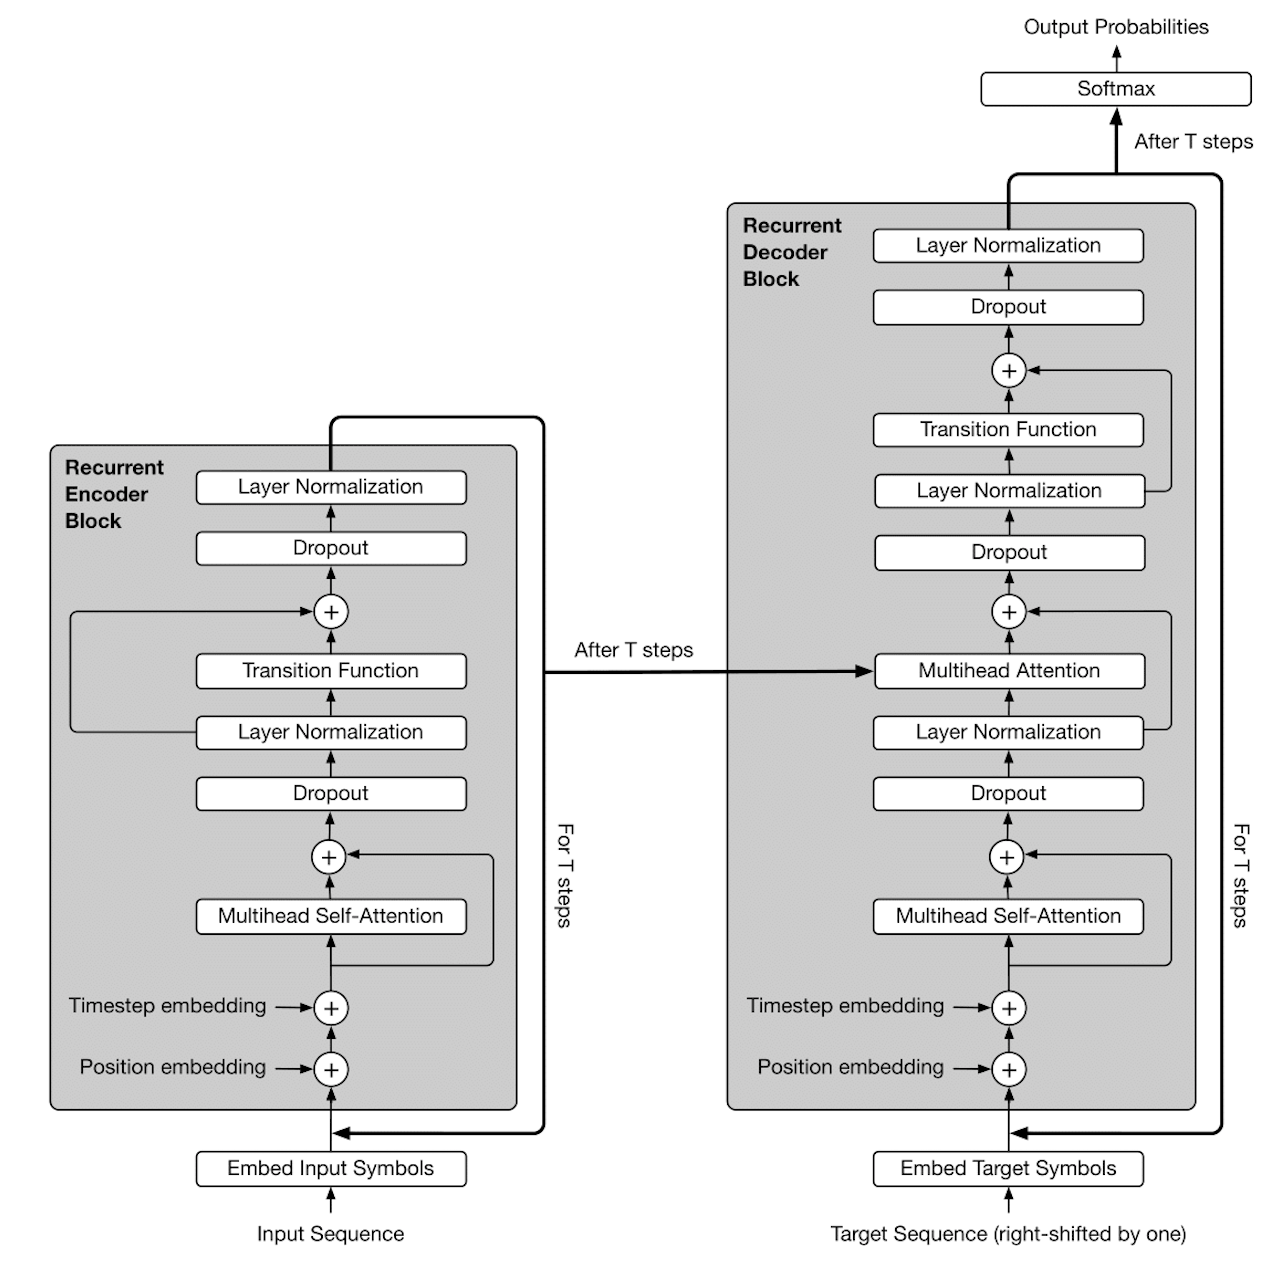
\includegraphics[height=.70\textwidth , width=.40\textwidth]{universal.png}
        \captionof{figure}{Universal Transformer }
\end{center}

\textbf{Decoder} is same as encoder except that it attends final encoder representation $H^T$ using the same multihead dot-product attention with query $Q$ obtained from decoder input representation and key and value pair $K, V$ using linear projection of $H^T$.\\
In sequence processing systems, few symbols are ambiguous than others. Consider the sentence \quotes{I arrived at the bank after crossing the river}. Here word \quotes{bank} is more ambigious compared to other words hence its reasonable to spend more processing resources for some words. Standard Transformer applies same amount of processing to every word unlike Universal Transformer. \\
Universal Transformer uses Adaptive Computation Time (ACT) \cite{DBLP:journals/corr/Graves16} mechanism to dynamically decide number of processing steps required to process input words in sequence. \\
Universal Transformer increases theoretical expressiblity of Transformer and makes it turing complete.
UT achieves new state of the art result on babI question answering task and  LAMBADA Language Modeling.
 	\section{Semi-Autoregressive Transformer }   
    Transformers are autoregressive, In the sense that they produce output one by one. Recently a group of Alibaba team proposed a model that can produce $K$ words at a time with not much compromising with accuracy, It gives tradeoff between accuracy and speed. Transformer can be viewed as special case of Semi-Autoregressive Transformer (SAT)\cite{wang2018semiautoregressive} when $K=1$. \\
    Any encoder-decoder architecture first encodes source sentence $x_1, x_2 \dots x_m$ into hidden states and then decoder generates target sentence $y_1, y_2 \dots y_n$ ates according to an autoregressive model
$p(y_t|y_1, y_2 \dots y_{t-1}, \textbf{x})$. \\
SAT extends word-level chain rule to the group-level chain rule.

  \noindent $p(y_1, y_2 \dots y_n \mid \textbf{x}) = {\displaystyle \prod_{t=1}^\floor*{\frac{(n-1)}{K}}+1} p(G_t|G_1, G_2 \dots G_{t-1}, \textbf{x}) $

    \noindent \resizebox{1\hsize}{!}{$G_1, G_2 \dots G_{\floor*{(n-1)/K}+1} = y_1, \dots y_k, y_{k+1} \dots y_{2k}, \dots y_{\floor*{(n-1)/K}\times K+1} \dots y_n$}
Here words in same group are independent and can be produced in parallel. \\
This way, SAT is able to perform long distance prediction. We feed $y_{t-k}$ to predict $y_t$.

\section{Self-Attention with Relative Position Representations}
Transformer uses absolute
positions to its input for positional encoding. Recent work by Shaw et. al. \cite{shaw2018selfattention}(one of the author of this paper is first author for Transformer paper )  shows that, we can modify transformer to capture  relative position representation for self-attention mechanism.

\begin{itemize}
    \item Self-Attention: \\
   Input sequence  $(x_1, x_2, ... , x_n)$ is passed through sublayers of encoder and mapped to  $(z_1, z_2, ... , z_n)$.
   \begin{center}
       $e_{ij} = \frac{1}{\sqrt{d_z}}(x_iW^Q)(x_jW^K)^T$
   \end{center}
   attention weight (alpha) is computed by softmax function-
    \begin{center}
      $\alpha _{ij} = \frac{\text{exp}e_{ij}}{\sum_{k=1}^{n} \text{exp}e_{ik}}$
   \end{center}
   These scores further getss multipy with \textbf{value} vectors to produce final token representation-
       \begin{center}
      $z_i = \sum_{j=1}^{n} \alpha _{ij}(x_jW^V)$
   \end{center}
   
   \item Relation aware self attention:- \\
   Shaw et al. \cite{shaw2018selfattention} proposed relation aware self attention in which edge information is added while keeping input and output same as Transformer.
    \begin{center}
       $e_{ij} = \frac{1}{\sqrt{d_z}}(x_iW^Q)(x_jW^K+a_{ij}^K)^T$
   \end{center}
  $\Big( \alpha _{ij}$ is same softmax function  $\alpha _{ij} = \frac{\text{exp}e_{ij}}{\sum_{k=1}^{n} \text{exp}e_{ik}}\Big)$ \\
  
  \noindent And final token representation is calculated using edge information too.
   \begin{center}
      $z_i = \sum_{j=1}^{n} \alpha _{ij}(x_jW^V+a_{ij}^V)$
   \end{center}
   maximum relative position is clipped to a max absolute value of k
 \begin{center}
      $ \alpha _{ij}^K = w_{\text{clip}(j-1,k)}^K$\\
       $ \alpha _{ij}^V = w_{\text{clip}(j-1,k)}^V$\\
       $ \text{clip}(x,k) = max(-k, min(k,x))$
   \end{center}
   On the WMT 2014 English-to-German and English-to-French translation tasks, this approach yields improvements of 1.3 BLEU and 0.3 BLEU over absolute position representations(Transformer), respectively.
\end{itemize}

    \bibliography{refere}
	
    \bibliographystyle{abbrv}
	
	\end{multicols}
\end{document}
